\section{Introduction}

\begin{definition}[\textit{Causal inference}]
    Causal inference is the process of identifying the independent and actual effect of a specific phenomenon within a larger system.
\end{definition}

It is crucial to emphasize that correlation does not imply causation.
\begin{example}
    Let's consider a new pandemic where we need to choose the most effective treatment among two possibilities.
    treatment $T=\{A,B\}$, condition $C=\{Mild,Severe\}$, and outcome $Y=\{Alive, Dead\}$ are the variables of interest. 
    The initial mortality rate table is presented below:
    \begin{table}[H]
        \centering
        \begin{tabular}{ccc}
        \hline
        \textbf{Treatment} & \textbf{Mortality} & \textbf{Proportion} \\ \hline
        $A$                & $16\%$             & $240/1500$  \\
        $B$                & $19\%$             & $105/550$   \\ \hline
        \end{tabular}
    \end{table}
    Initially, treatment $A$ seems preferable as it exhibits a lower mortality percentage.
    However, introducing patient condition data alters the assessment:
    \begin{table}[H]
        \centering
        \begin{tabular}{|c|cc|cccc|}
        \hline
        \textbf{Treatment} & \multicolumn{2}{c|}{\textbf{Total}} & \multicolumn{2}{c}{\textbf{Mild}} & \multicolumn{2}{c|}{\textbf{Severe}} \\ \hline
        $A$                & $16\%$         & $240/1500$         & $15\%$        & $210/1400$        & $30\%$          & $30/100$           \\
        $B$                & $19\%$         & $105/550$          & $10\%$        & $5/50$            & $20\%$          & $100/500$          \\ \hline
        \end{tabular}
    \end{table}
    Surprisingly, with this updated table, treatment $B$ emerges as the superior choice, leading to a paradox known as Simpson's paradox.
    This paradox results from the unequal distribution of patients across treatments.

    To address this paradox, considering different treatments for mild and severe patients may be a solution. 
    Two scenarios are explored:
    \begin{enumerate}
        \item Assigning treatment $A$ to mild patients and treatment $B$ to severe patients. 
            The corresponding causality graph is as follows:
            \begin{figure}[H]
                \centering
                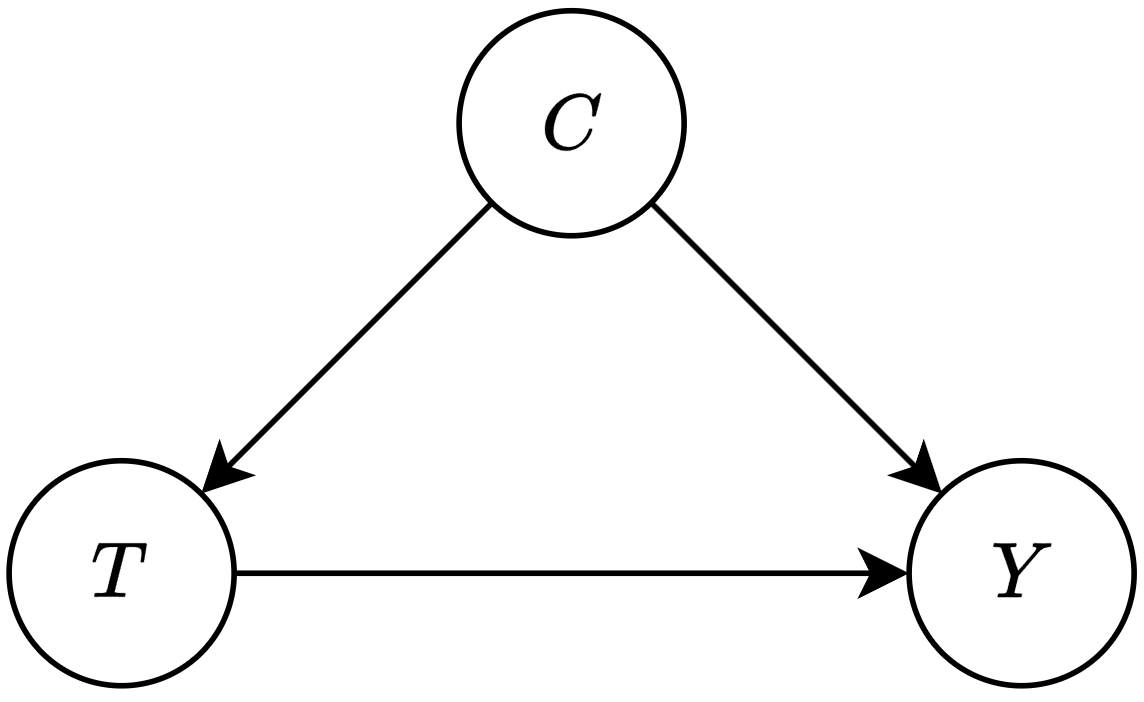
\includegraphics[width=0.25\linewidth]{images/cau.png}
            \end{figure}
        \item Prioritizing mild patients with treatment $A$ due to its quick availability, while administering the slower treatment $B$ to severe patients.
        The corresponding causality graph is illustrated below:
            \begin{figure}[H]
                \centering
                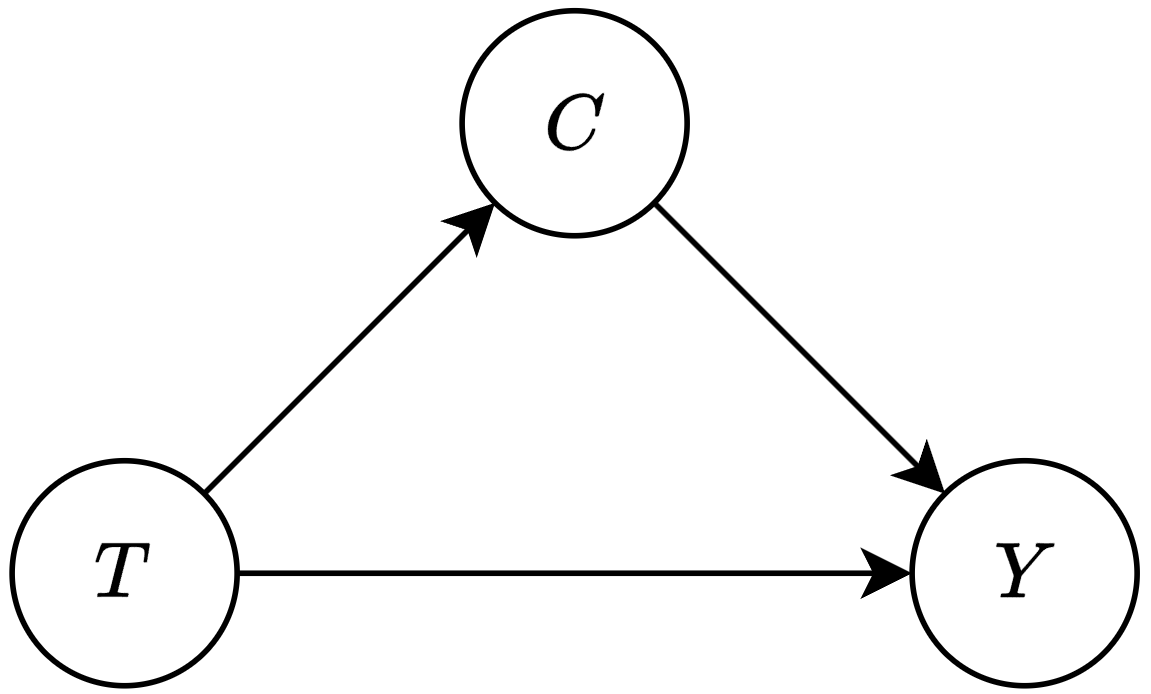
\includegraphics[width=0.25\linewidth]{images/cau1.png}
            \end{figure}
    \end{enumerate}
    Notably, the choice of treatment is influenced by the underlying causality graph.
\end{example}

To assess the correlation between two events, we can choose to either implement or abstain from the action causing the event.
In the former case, we refer to it as factual evidence, while in the latter, it constitutes counterfactual evidence.
The causal effect is quantified as the difference between factual and counterfactual evidences:
\[Y_i(1)-Y_i(0)=1\]
\begin{definition}[\textit{Individual treatment effect}]
    The individual treatment effect is defined as the disparity between taking an action and doing nothing within a population:
    \[Y_i(1)-Y_i(0)\]
\end{definition}
\begin{definition}[\textit{Average treatment effect}]
    The average treatment effect is defined as the expected value of the individual treatment effect:
    \[\mathbb{E}\left[Y_i(1)-Y_i(0)\right]=\mathbb{E}\left[Y_i(1)\right]-\mathbb{E}\left[Y_i(0)\right] \neq \mathbb{E}\left[ Y\mid T=1 \right]-\mathbb{E}\left[ Y\mid T=0 \right]\]
\end{definition}
The inequality in the previous definition arises from the distinction that the first term considers only causal associations, while the second term includes both causal and confounding associations.

\paragraph*{Randomized control trials}
A potential remedy to this challenge is to address confounding associations through randomized control trials
In RCTs, subjects are randomly assigned to treatment groups, ensuring that $T$ does not have causal parents, and the groups are comparable.
However, the applicability of this technique may be limited due to ethical concerns, infeasibility, or outright impossibility.
\begin{figure}[H]
    \centering
    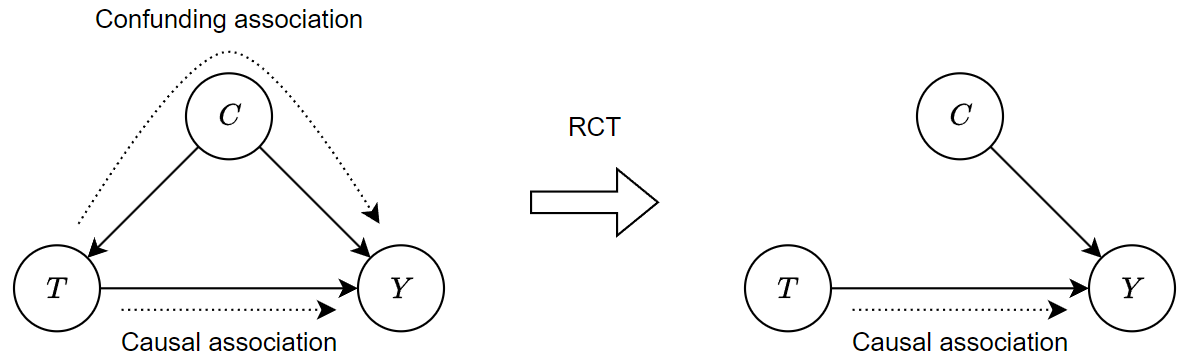
\includegraphics[width=0.75\linewidth]{images/cau2.png}
    \caption{Differences between base case and RCT case}
\end{figure}

\paragraph*{Confounding adjustments}
An alternative strategy is to control for the appropriate variables $W$. 
If $W$ forms a sufficient adjustment set, we can express:
\[\mathbb{E}\left[Y(t)\mid W=w\right]=\mathbb{E}\left[Y\mid T=t,W=w\right]=\mathbb{E}\left[Y\mid t,w\right]\]
By marginalizing $W$, we arrive at the backdoor adjustment formula:
\[\mathbb{E}\left[Y(t)\right]=\mathbb{E}\left[Y\mid T=t\right]=\mathbb{E}_W\left[Y\mid t,W\right]\]
It is important to note that the set of variables leading to d-separation acts as a sufficient adjustment set.
\begin{figure}[H]
    \centering
    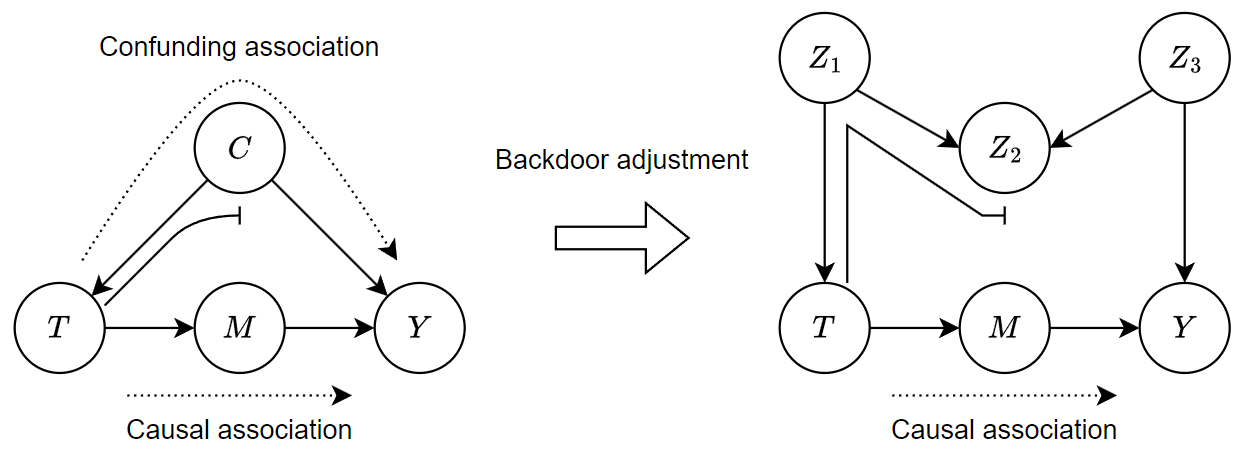
\includegraphics[width=0.75\linewidth]{images/cau3.png}
    \caption{Differences between base case and RTC case}
\end{figure}
\begin{example}
    Consider Simpson's paradox illustrated by the mortality table:
    \begin{table}[H]
        \centering
        \begin{tabular}{|c|cc|cccc|}
        \hline
        \textbf{Treatment} & \multicolumn{2}{c|}{\textbf{Total}} & \multicolumn{2}{c}{\textbf{Mild}} & \multicolumn{2}{c|}{\textbf{Severe}} \\ \hline
        $A$                & $16\%$         & $240/1500$         & $15\%$        & $210/1400$        & $30\%$          & $30/100$           \\
        $B$                & $19\%$         & $105/550$          & $10\%$        & $5/50$            & $20\%$          & $100/500$          \\ \hline
        \end{tabular}
    \end{table}
    Let's consider the first scenario, leading to the following Bayesian network:
    \begin{figure}[H]
        \centering
        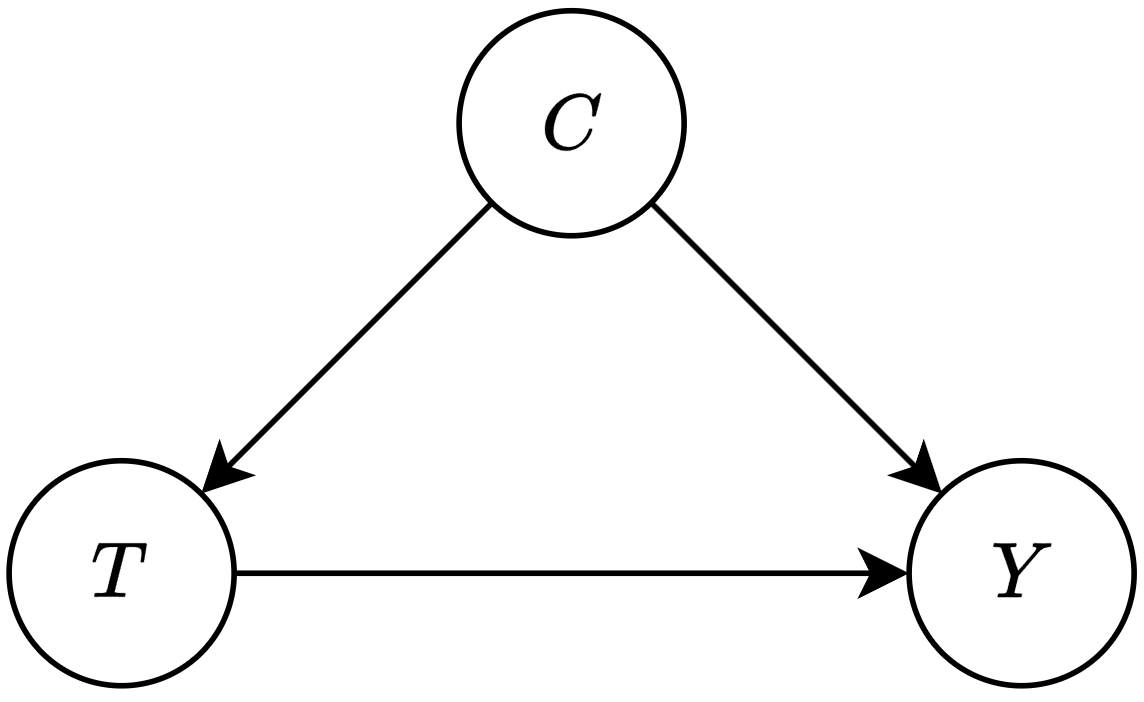
\includegraphics[width=0.25\linewidth]{images/cau.png}
    \end{figure}
    Choosing treatment $A$ based on the total percentage is inaccurate due to the uneven distribution of mild and severe cases. 
    To make the best decision, we break the confounding correlation:
    \[\mathbb{E}\left[Y\mid T=t\right]=\mathbb{E}_C\left[Y\mid t,C\right]=\sum_C\mathbb{E}\left[ T\mid t,c \right]\Pr(c)\]
    Normalizing the number of people checked, we obtain:
    \[\Pr_{\text{causal}}(A)=\dfrac{1450}{2050}(0.15)+\dfrac{600}{2050}(0.30)=0.194\]
    \[\Pr_{\text{causal}}(B)=\dfrac{1450}{2050}(0.10)+\dfrac{600}{2050}(0.20)=0.129\]
    In contrast, the naïve probabilities were:
    \[\Pr_{\text{naïve}}(A)=\dfrac{1400}{1500}(0.15)+\dfrac{100}{1500}(0.30)=0.16\]
    \[\Pr_{\text{naïve}}(B)=\dfrac{50}{550}(0.10)+\dfrac{500}{550}(0.20)=0.19\]
\end{example}